\section{Method}

Our method takes as input an existing oversegmentation of an $EM$ image volume. 
Section~\ref{sec:neuroproof} discusses two preexisting pipelines for generating these segmentations.
We evaluate our proposed method on the outputs from both of these pipelines.

\subsection{Graph Creation}

We need to generate nodes $N$ and edges $E$ to apply a graph-based optimization strategy for segmentation. 
In addition, these edges need non-negative weights.

\subsubsection{Node Generation}

The simplest node generation strategy creates one node for every unique segment label in the input volume.
However, there are often a small number of labels in the volume corresponding to very small regions.
It is difficult to extract useful shape features from these segments because of their small, and often random, shape. 
These segments are pruned from the graph and do not have corresponding nodes. 
For the proposed framework, we remove segments with fewer than $20,000$ voxels (ADD PERCENT, current estimate less than 10\%).
Figure~\ref{fig:skeletonization} shows two typical input segments that receive a corresponding node in the graph. . 

\subsubsection{Edge Generation}

\begin{figure}[t]
	\centering
	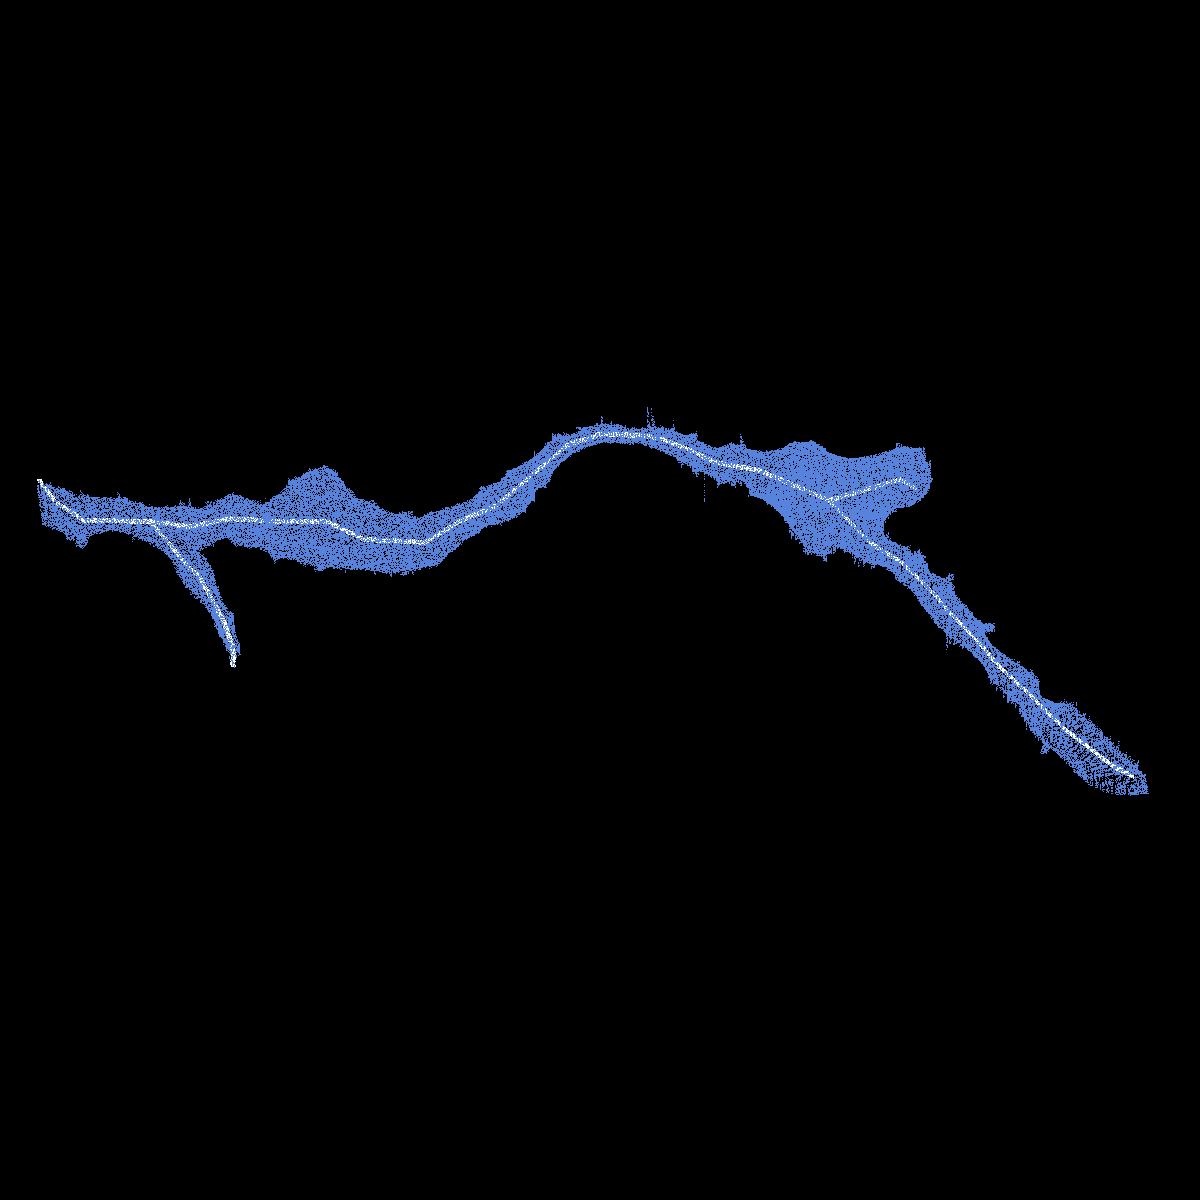
\includegraphics[width=0.42\linewidth]{./figures/skeleton1.png}
	\hspace{0.085\linewidth}
	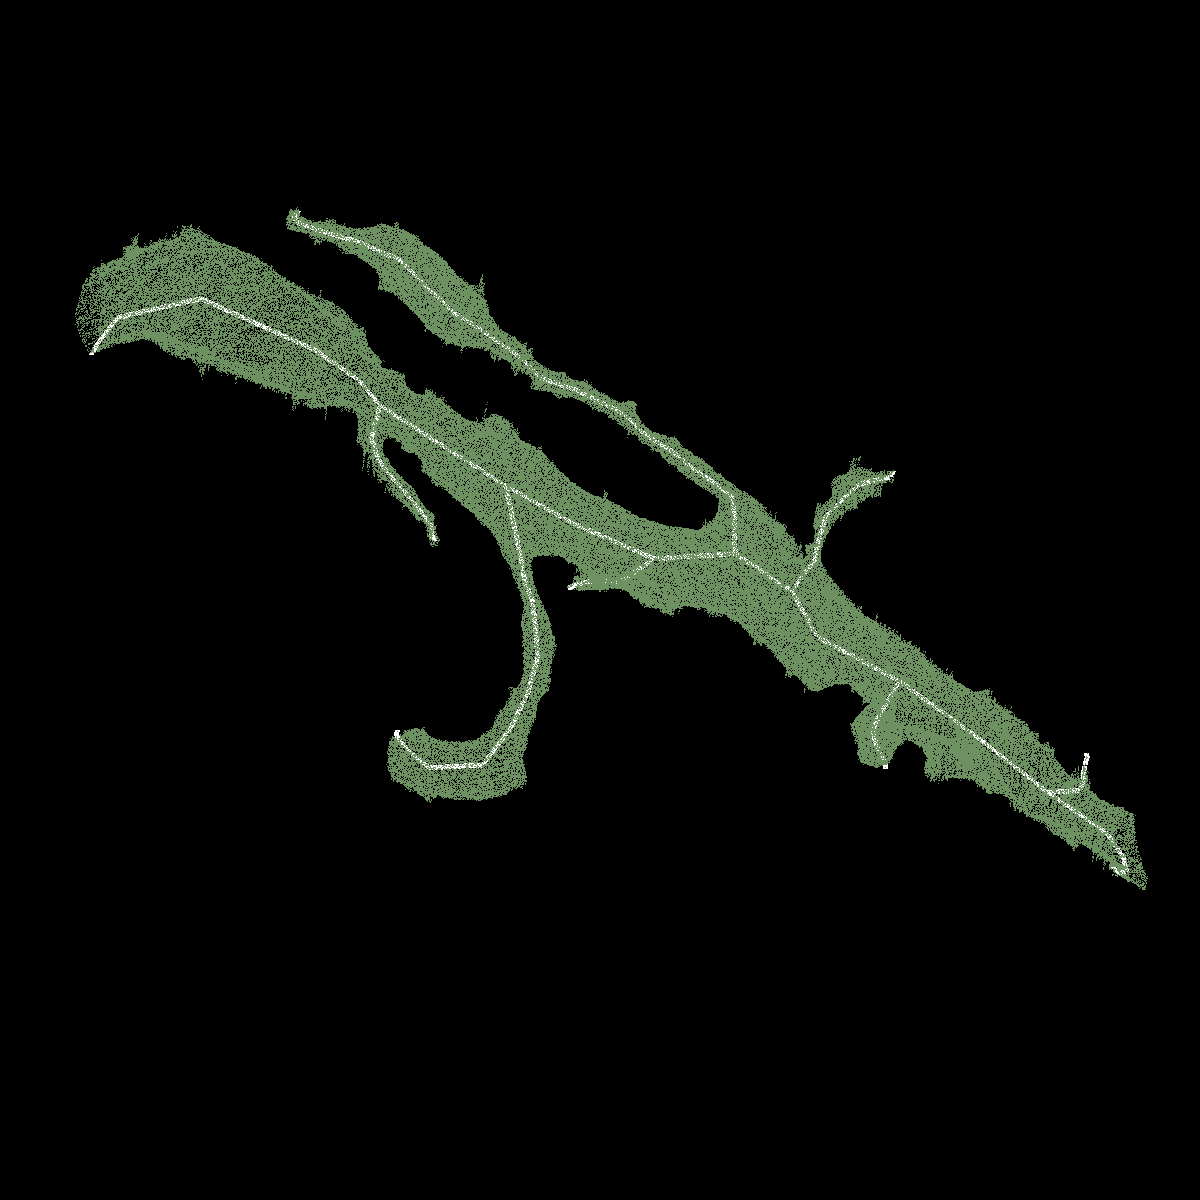
\includegraphics[width=0.42\linewidth]{./figures/skeleton2.png}
	\caption{Two example outputs of the TEASER skeletonization algorithm.}
	\label{fig:skeletonization}
\end{figure}

A na\"ive approach to generating edges simply produces an edge between all segments that have a single pair of neighboring voxels.
Current agglomeration strategies such as NeuroProof or GALA use this criteria when deciding pairs of segments to merge into one neuron.
However, for us this method will produce too many edges in our graph, many of which are easily prunable. 
Many of the segments that are erroneously split have a similar structure. 
Consider Figure~\ref{fig:merge_candidates} which shows two such pairs.
In both instances the segments around the break follow the same general shape. 
The segment is tubular in the close vicinity with an abrupt break perpendicular to the elongated direction.
We present the following algorithm to identify these locations.

We generate a skeleton for every segment following the intuition that a skeleton represents a simplified representation of the overall shape of an object. 
We use the Tree-structure Extraction Algorithm for Accurate and Robust Skeletons (TEASER)~\cite{sato2000teasar,zhao2014automatic}. 
These skeletons consist of a sequence of \textit{joints} with edges between successive joints. 
We prune the joints that are within $50$ voxels of each other to reduce unnecessary branching.
For the purposes of this algorithm, joints that have only one connected neighbor are referred to as \textit{endpoints}. 
Figure~\ref{fig:skeletonization} shows the skeletons in white of two typical segments from the label volume.
After skeletonization, we begin to identify segments for merge consideration with the following two-pass heuristic.
In the first pass, we iterate over all endpoints $e$ belonging to a segment $S$ and create a set of segments $\mathbb{S}_e^\prime$ which includes all labels that have a single voxel within $t_{low}$ nanometers from $e$. 
This first pass often includes too many candidates that should not merge so we apply an additional pass to prune these sets.
In the second pass, we consider all of the segments $\mathbb{S}_e^\prime$ for every endpoint $e$. 
If a segment $S^\prime \in \mathbb{S}_e^\prime$ has an endpoint within $t_{high}$ nanometers of $e$, the segment $S$ and $S^\prime$ are considered for merging. 
We store the midpoint between the two endpoints as the ``center" of the potential merge.
Algorithm (ADD REF) provides pseudocode for this edge generation algorithm. 
The results in this paper follow from $t_{low} = 240$ and $t_{high} = 600$. 

\begin{figure}[t]
	\centering
	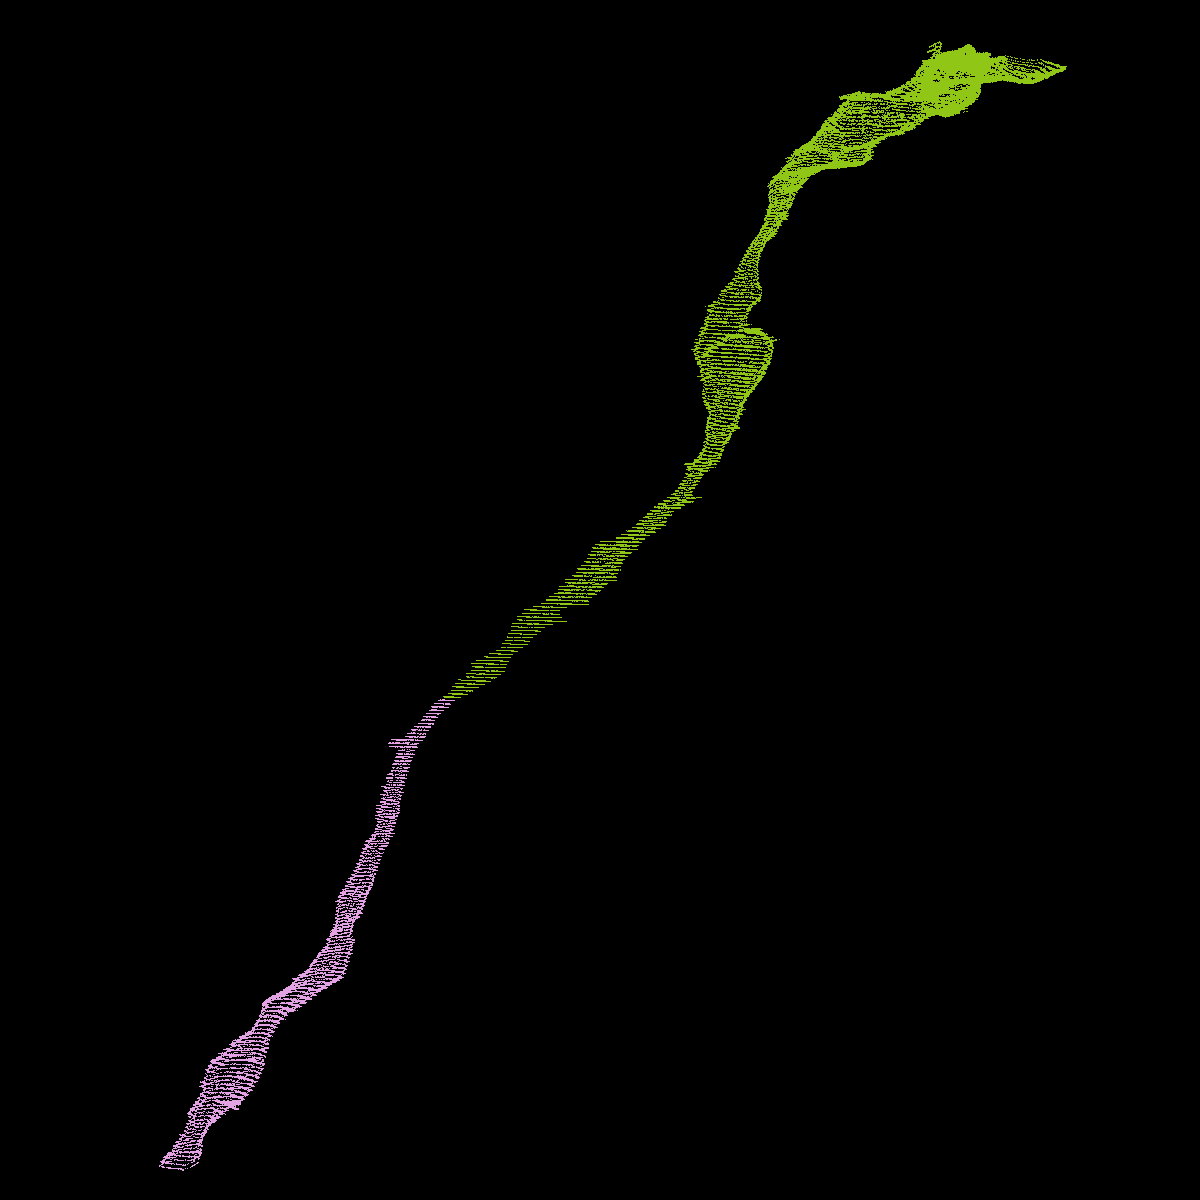
\includegraphics[width=0.42\linewidth]{./figures/merge_candidate1.png}
	\hspace{0.085\linewidth}
	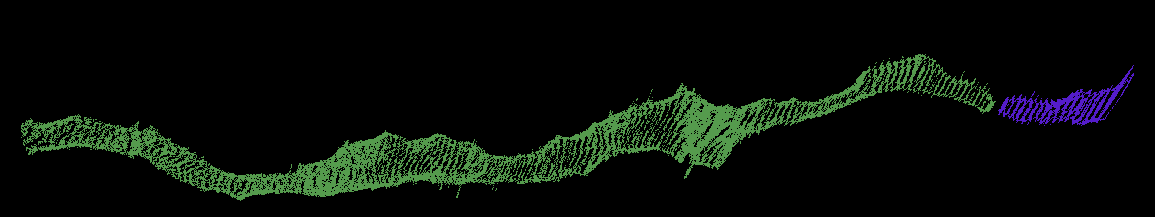
\includegraphics[width=0.42\linewidth]{./figures/merge_candidate2.png}
	\caption{Two erroneously split segments that should merge together. Most segments that we want to merge have the same general structure.}
	\label{fig:merge_candidates}
\end{figure}


\begin{algorithmic}
	\Function{GenerateEdges}{$skeletons$}
		\For {$skeleton$ in $skeletons$}
			\State $candidates$ = set()
			\For {$endpoint$ in $skeleton$}
				\State TODO ADD CODE
			\EndFor
		\EndFor
	\EndFunction
\end{algorithmic}

Note that the above algorithm does not enforce any segment adjacency constraints.
Figure (ADD FIGURE) shows two examples that would not be considered in previous research since they are not adjacent.
Finding and merging these examples is one of the benefits of retreating from per-pixel algorithms. 

\subsection{Edge Probabilities}

The previous section outlines how to generate edges between nodes in our graph structure. 
Here we introduce a neural network architecture for generating probabilities that two nodes sharing an edge belong to the same neuron. 
The neural network takes as input only data from the input segmentation. 

\subsubsection{Network Architecture}

\begin{figure*}[t]
	\centering
	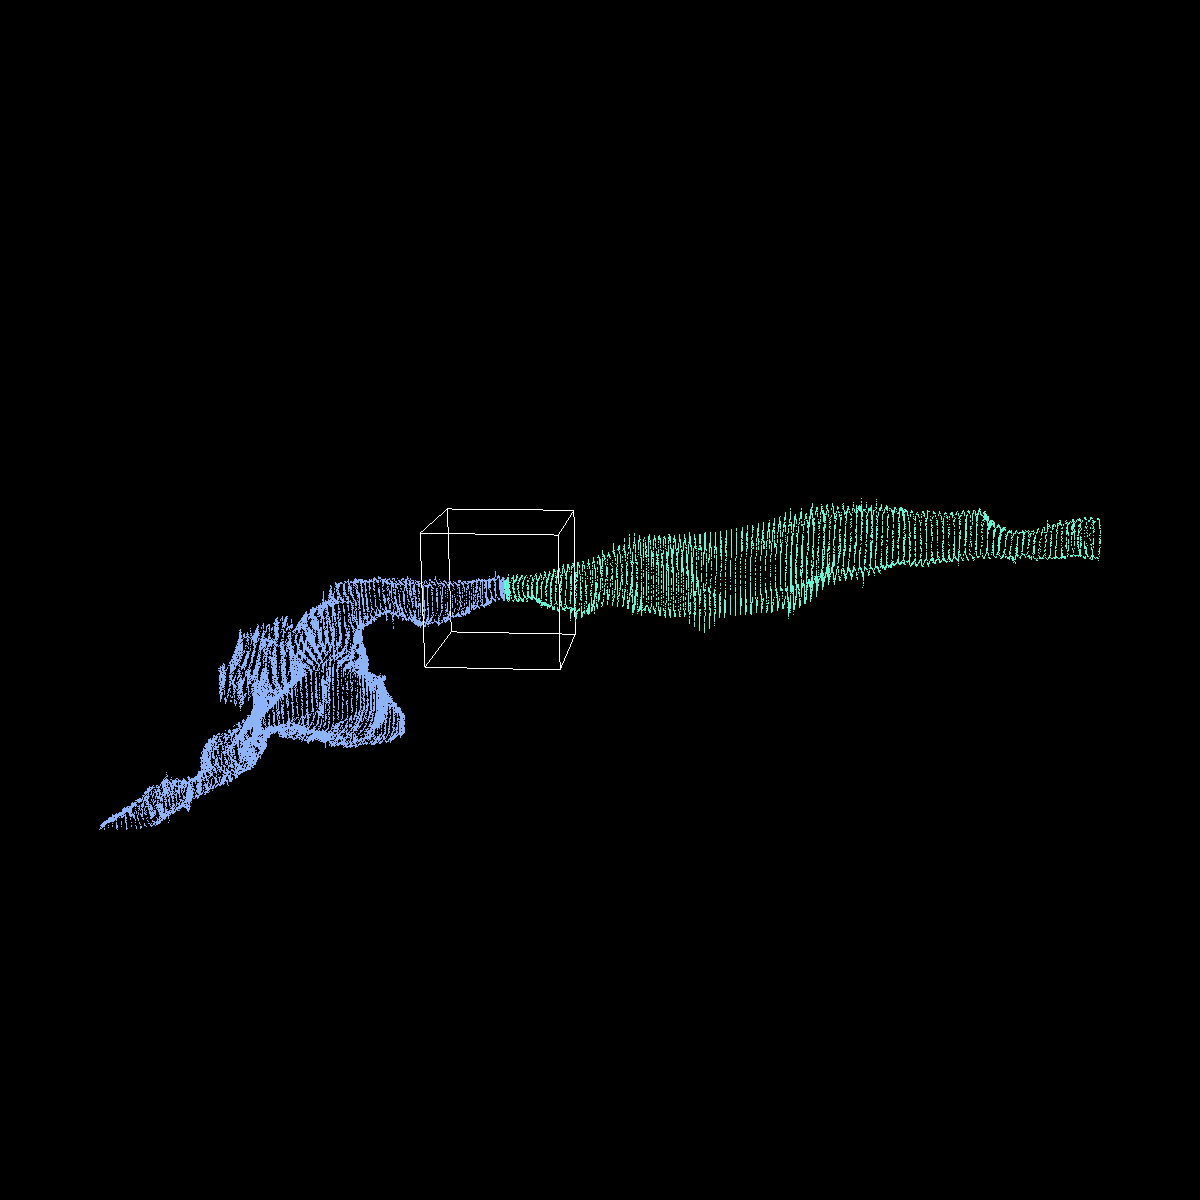
\includegraphics[width=0.3\linewidth]{./figures/network_distance_400.png}
	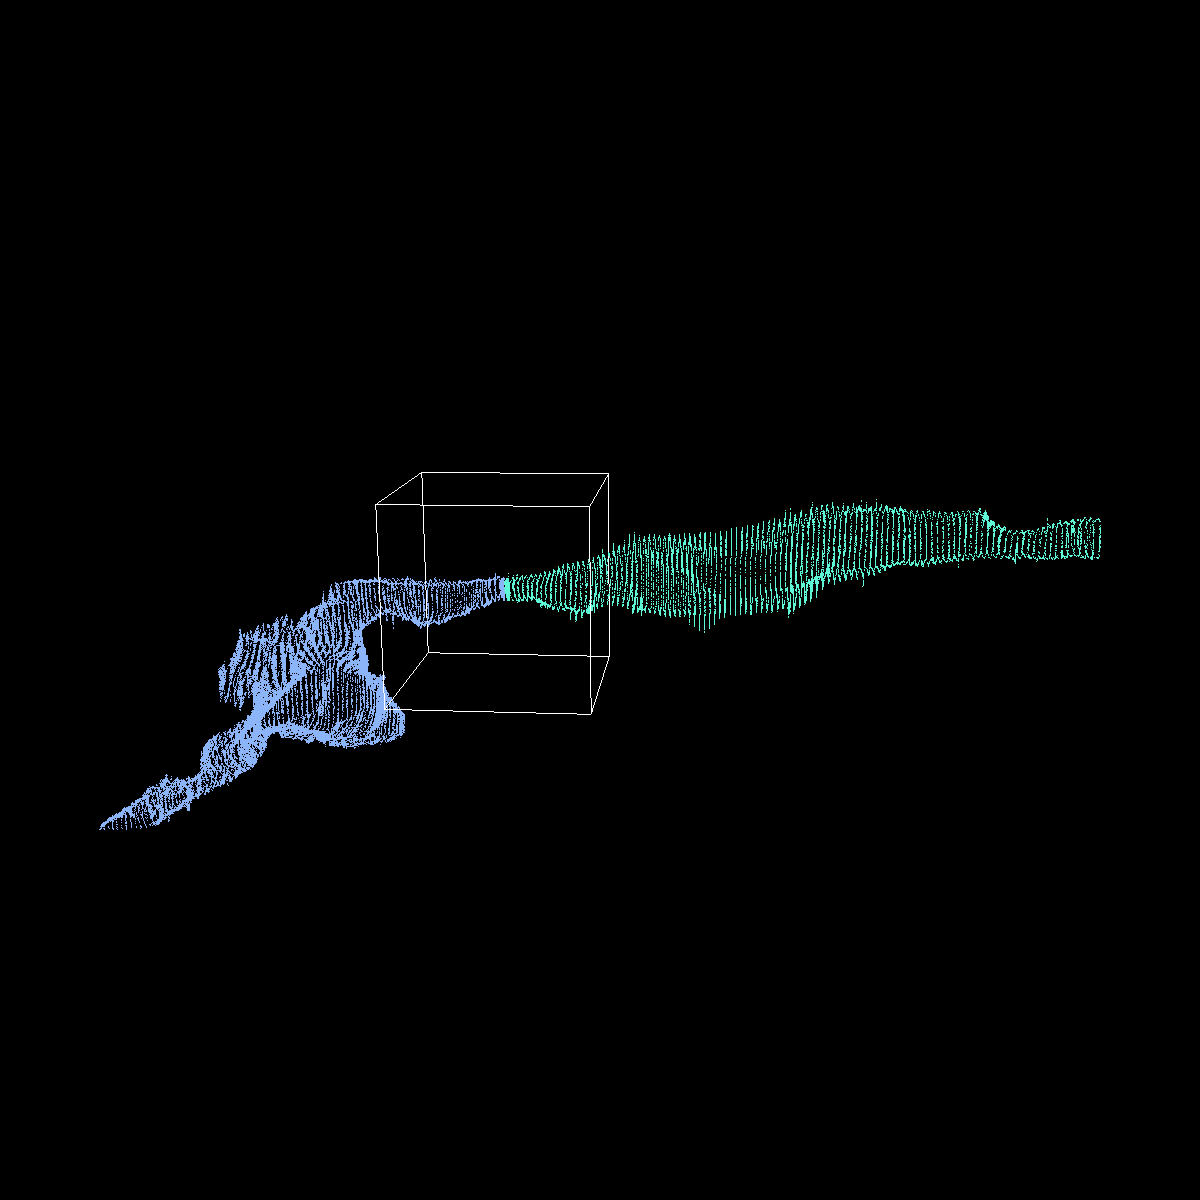
\includegraphics[width=0.3\linewidth]{./figures/network_distance_600.png}
	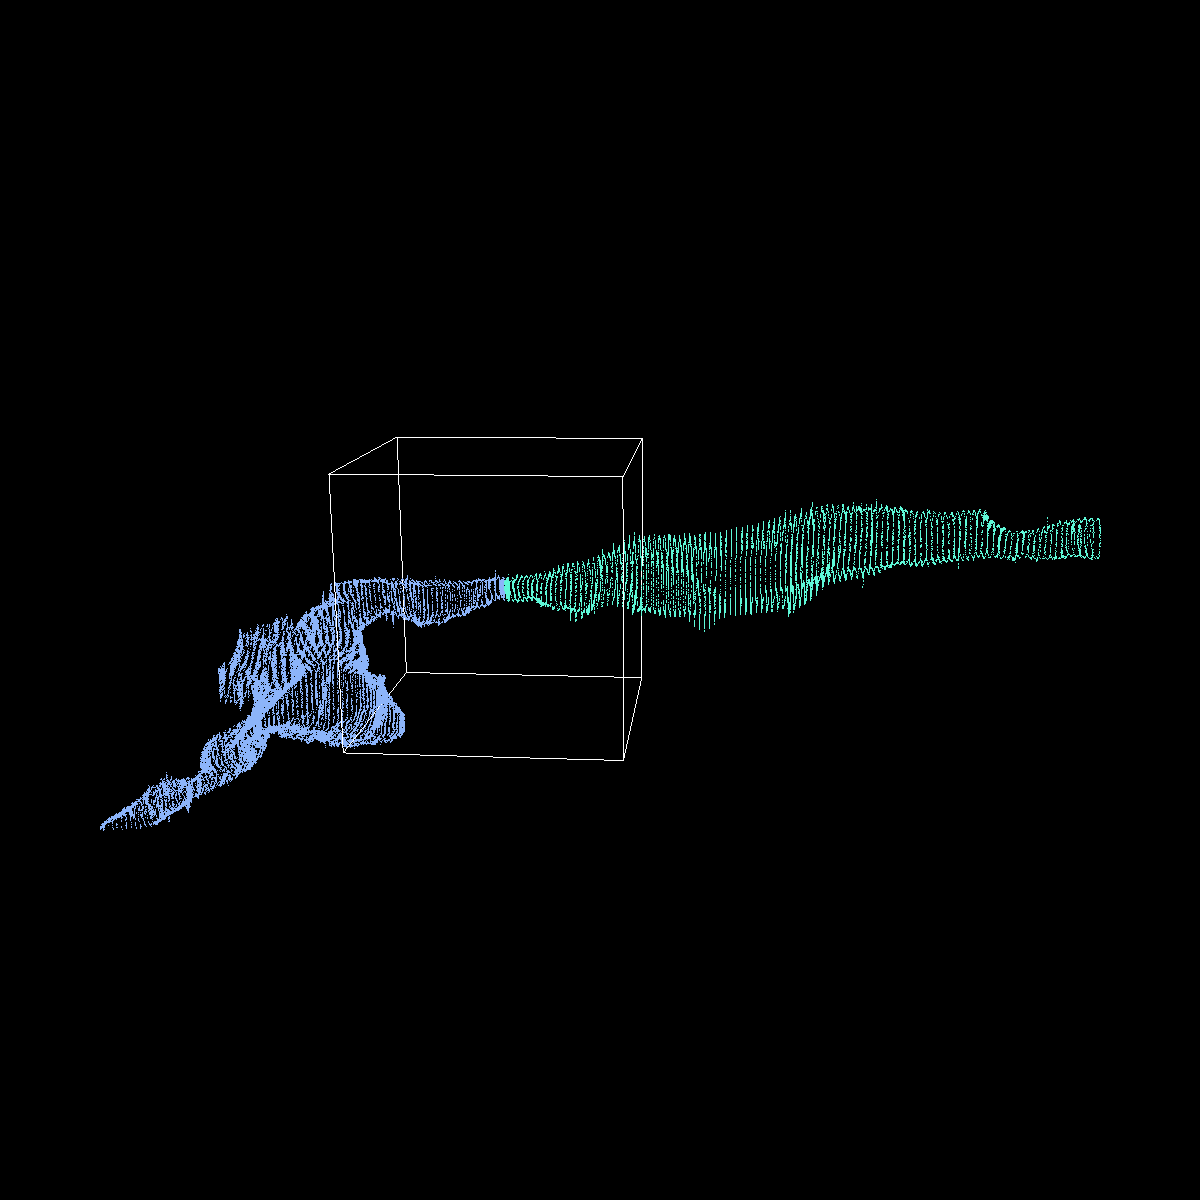
\includegraphics[width=0.3\linewidth]{./figures/network_distance_800.png}	
	\caption{The white outlines show three different possible cubic sizes to input into the neural network. The left example ($800\textrm{nm}$) provides less local context than the middle example ($1200\textrm{nm}$). The right example ($1600\textrm{nm}$) extracts too large of a local region that produces noise as one of the segments leaves the bounding box only to reenter.}
	\label{fig:network-radius}
\end{figure*}


The above skeletonization algorithm produces 3-D locations that require further consideration for merging. 
To determine which of these segments should actually merge, we train a 3-D convolutional neural network. 
We extract a cubic region with length $1200\textrm{nm}$ centered at these locations. 
These cubes will provide the local information for the neural network to predict which neighboring segments belong to the same neuron. 
A cubic length of $1200\textrm{nm}$ provides enough local shape context for the network without introducing an excessive amount of noise. 
Figure~\ref{fig:network-radius} shows cubes of lengths $800\textrm{nm}, 1200\textrm{nm},$ and $1600\textrm{nm}$.

We transform the extracted cubes for input into the neural network. 
The network takes three input channels for each voxel in the 3-D volume corresponding to the following mapping. 
Consider a pair of segments with labels $l_1$ and $l_2$ for every voxel $v$ in the cube of interest. 
The first channel is $0.5$ if $v = l_1$ and $-0.5$ otherwise, the second channel is $0.5$ if $v = l_2$ and $-0.5$ otherwise, and the third channel is $0.5$ if $v = l_1$ or $v = l_2$ and $-0.5$ otherwise. 
Each 3-channel volume is subsequently downsampled into an array of size $(3, 22, 68, 68)$ using nearest-neighbor interpolation. 
Our neural network trains on these 4-D arrays to generate probabilities that $l_1$ and $l_2$ should merge.

Our network architecture has three layers of double convolutions followed by a max pooling step \cite{chatfield2014return}. 
As described above, the input with into the network is $(22, 68, 68)$ with $3$ channels. 
The filter size of the layers are 16, 32, and 64 with size doubling deeper into the network. 
The first two max pooling layers are anisotropic with pooling only in $x$ and $y$ to match the anisotropic nature of our EM datasets. 
All convolutions have kernel sizes of $(3, 3, 3)$. 
The output size of the final max pooling layer is $(5, 5, 5)$ with $64$ channels. 
The output is flattened into a 1-D vector with $8000$ entries which enters two fully connected layers with $512$ and $1$ dimensions in the output respectively. 
All activation functions are LeakyReLU with $\alpha=0.001$ except for the final activation which uses a sigmoid function~\cite{funahashi1989approximate,maas2013rectifier}. 
There is a dropout of $0.2$ after every pooling layer and the first dense layer. 
There is a dropout of $0.5$ after the final dense layer. 
The above method uses stochastic gradient descent with Nesterov's accelerated gradient~\cite{nesterov1983method}. 
This optimizer has an initial learning rate of $0.01$, momentum of $0.9$, and a decay rate of $5*10^{-8}$. Figure~\ref{fig:architecture} provides an overview of the proposed architecture. 

\begin{figure*}[t]
	\centering
	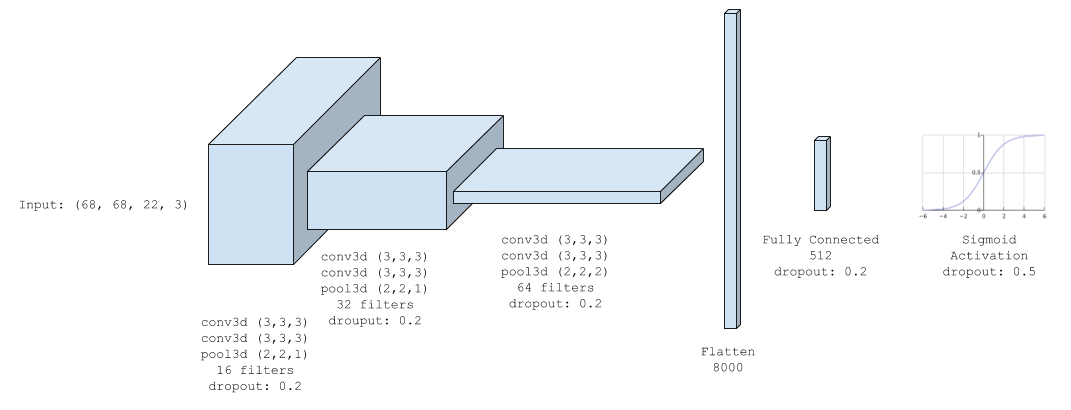
\includegraphics[width=0.95\linewidth]{figures/architecture.png}
	\caption{The architecture for the neural networks follows the \textit{VGG} style of double convolutions followed by a max pooling operation. The number of filters doubles each layer leading to a fully connected layer and a sigmoid activation function.}
	\label{fig:architecture}
\end{figure*}


\subsubsection{Data Augmentation}

We apply some data augmentation to the generated examples to increase the size of the training datasets. 
We consider all rotations of $90$ degrees along the $xy$-plane in addition to mirrors along the $x$ and $z$ axes. 
This produces an additional 16 times more training data. 

\subsection{Agglomeration}

After constructing the above graph structure we can apply a graph-based segmentation strategy. 
There are many formulations of graph-based optimization strategies that provide different guarantees on their output. 
Neurons in the brain should be acyclic, i.e. the output shape should have a genus of zero. 
Current connectomics agglomeration techniques do not leverage this additional information but rather consider neighboring regions in successive order without regard to loop creation. 
In our graph formulation we can enforce this topological property by applying a multicut partition onto the graph which generates a forest on the nodes. 
There are several heuristics that solve the multicut problem. For our purposes we use the Kernighan-Lin algorithm~\cite{kernighan1970efficient}.